\documentclass[12pt]{article}
\usepackage[top=1in,left=1in, right = 1in, footskip=1in]{geometry}

\usepackage{graphicx}
%\usepackage{adjustbox}

\newcommand{\eref}[1]{(\ref{eq:#1})}
\newcommand{\fref}[1]{Fig.~\ref{fig:#1}}
\newcommand{\Fref}[1]{Fig.~\ref{fig:#1}}
\newcommand{\sref}[1]{Sec.~\ref{#1}}
\newcommand{\frange}[2]{Fig.~\ref{fig:#1}--\ref{fig:#2}}
\newcommand{\tref}[1]{Table~\ref{tab:#1}}
\newcommand{\tlab}[1]{\label{tab:#1}}
\newcommand{\seminar}{SE\mbox{$^m$}I\mbox{$^n$}R}

\usepackage{amsthm}
\usepackage{amsmath}
\usepackage{amssymb}
\usepackage{amsfonts}

\usepackage{lineno}
%\linenumbers

\usepackage[pdfencoding=auto, psdextra]{hyperref}

\bibliographystyle{chicago}
\usepackage{natbib}
\date{\today}

\usepackage{xspace}
\newcommand*{\ie}{i.e.\@\xspace}

\usepackage{color}

\newcommand{\Rx}[1]{\ensuremath{{\mathcal R}_{#1}}} 
\newcommand{\Ro}{\Rx{0}}
\newcommand{\RR}{\ensuremath{{\mathcal R}}}
\newcommand{\Rhat}{\ensuremath{{\hat\RR}}}
\newcommand{\tsub}[2]{#1_{{\textrm{\tiny #2}}}}

\newcommand{\comment}[3]{\textcolor{#1}{\textbf{[#2: }\textsl{#3}\textbf{]}}}
\newcommand{\jd}[1]{\comment{cyan}{JD}{#1}}
\newcommand{\swp}[1]{\comment{magenta}{SWP}{#1}}
\newcommand{\dc}[1]{\comment{blue}{DC}{#1}}
\newcommand{\hotcomment}[1]{\comment{red}{HOT}{#1}}

\newcommand{\jdnew}{\jd{NEW}}
\newcommand{\jddel}[1]{\jd{DELETE: #1}}

\begin{document}

\begin{flushleft}{
	\Large
	\textbf\newline{
		The role of community transmission in driving the spread of SARS-CoV-2 on a university campus: lessons from Princeton University
	}
}
\newline
\\ 

\end{flushleft} 

\pagebreak

Predicting and controlling the spread of SARS-CoV-2 remains a critical public health and scientific question.
Rapid, asymptomatic transmission of SARS-CoV-2 has hindered intervention efforts such as contact tracing.
Stringent measures to limit social contacts have been effective in preventing transmission in the beginning of the pandemic but are unsustainable.
The recent development of vaccines have provided a safe means of reopening the society, but uncertainty remains in their long-term effectiveness in protecting infection and transmission.
In addition, as new variants continues to emerge and 

the emergence of new variants, which can evade immunity and transmit better, continues to pose additional challenges.


Since the beginning of the pandemic, mathematical models have played a key role in evaluating intervention measures and guiding pandemic response.



testing has played a key role in monitoring and controlling the spread.
In addition, a frequent testing of a large fraction of the population, followed by rapid isolation and contact tracing, has proven effective in preventing chains of transmission and reducing the spread in large congregate settings.

University campuses provide unique test case in a relatively well-controlled setting for evaluating the feasibility of safe reopening.
High density environments and large fraction of asymptomatic infections (due to young age of university students) can readily permit rapid transmission.




- Usual pandemic start

- modeling, understanding control
- testing frequency is important
- universities provide a particularly test case; asymptomatic infection and testing is very high

- little review of what other universities have done

- epideimc in relatively well controlled documented setting
- really well until omicron
- perhaps because of immunity waning 

In this study, we analyze the spread of SARS-CoV-2 on Princeton University campus (\fref{princeton}).
Princeton University is located in Mercer County, New Jersey, USA and consists of roughly 5000 undergraduate students, 3000 graduate students, and 7000 faculty and staff members.
For simplicity, we divide the epidemic into three time periods representing four semesters: Fall 2020 (August 24, 2020--January 1, 2021; \fref{princeton}A), Spring 2020 (January 16, 2021--May 14, 2021; \fref{princeton}B), and Fall and Winter 2021 (August 14, 2021--January 14, 2021; \fref{princeton}C).
Throughout the study period, all students, faculty and staff members who were physically present for more than 8 hours on campus per week were required to participate in asymptomatic testing with varying frequencies.
Asymptomatic individuals submitted self-collected saliva samples, from which the presence of SARS-CoV-2 was tested using Reverse Transcription Polymerase Chain Reaction (RT-PCR).  
Asymptomatic individuals who tested positive were required to isolate for 10 days.
Symptomatic individuals were eligible for rapid PCR tests and had to isolate \swp{self-isolate?} until they received their test results---those who tested positive were required to isolate for at least 10 days after symptom onset and were release 3 days after symptoms resolved.
Those who tested positive were exempt from asymptomatic testing for 90 days.
Throughout the study period, contact tracing was also performed for positive cases to quarantine their close contacts, which refer to individuals who have been within 6 feet for at least 15 minutes, cumulatively within a 24-hour period.
All data used in this analysis are publicly available on Princeton University COVID-19 Dashboard website: \url{https://covid.princeton.edu/dashboard}.


\begin{figure}[!th]
\includegraphics[width=\textwidth]{../figure_princeton/figure_princeton.pdf}
\caption{
\textbf{Dynamics of SARS-CoV-2 outbreaks in Princeton University}
(A--C) Epidemic trajectories across three semesters: Fall 2020 (A), Spring 2020 (B), and Fall 20201 (C).
Colored bar plots represent the weekly number of cases from both asymptomatic and symptomatic testing in Princeton University.
Red lines represent the weekly number of cases in Mercer County.
Number of cases in Mercer County is obtained from \url{https://github.com/nytimes/covid-19-data}.
(D--F) Correlations between the weekly number of cases in Princeton University and in Mercer County.
Solid lines and shaded areas represent the estimated linear regression lines and the associated 95\% CIs.
\label{fig:princeton}
}
\end{figure}

During fall 2020, roughly 1000 grad students and 2000 faculty and staff members were present on campus and participated in asymptomatic testing. 
Undergraduate students were not allowed to return back to campus as all classes were held virtually, and so their numbers were minimal on campus ($<300$).  
Both undergraduate students and graduate students were required to get tested twice a week, whereas faculty and staff members were required to get tested once a week.
The number of cases remained relatively low throughout the semester with a peak occurring in early December, coinciding with the epidemic trajectory in Mercer County (\fref{princeton}A).  
A sudden decrease in the number of cases around Thanksgiving partly reflects the reduced number of tests (3852 and 2972 asymptomatic tests performed on the week ending November 20th and 27th, respectively).
The highest number of cases was reported among faculty and staff members (169), followed by graduate students (41), and undergraduate students (4).

In the beginning of spring 2020, the number of cases suddenly increased before classes began (\fref{princeton}B), reflecting $\approx 3000$ undergraduate students returning to campus.
Returning students were required to be tested and quarantine \swp{for how long} if they were coming back from CDC-designated states \swp{not sure if this is the right wording... but I remember we had a rule like this... we can ask Irini and Robin for this}.
All classes remained virtual, and the testing protocol did not change (twice a week for undergraduate and graduate students, and once a week for faculty and staff members).
The number of cases persisted at similar levels as the fall semester and eventually decreased as classes ended and students went back home---the decrease in the number of cases in Princeton University also coincided with the decrease in the number of cases in Mercer County.
The highest number of cases was reported among faculty and staff members (111), followed by undergraduate students (101), and graduate students (29).

In fall 2021, all students and faculty and staff members were required to be vaccinated \swp{with two doses? need to ask Robin} with a very few medical and religious exemptions.
By the beginning of the semesters, ??\% of students and ??\% of faculty and staff members were vaccinated \swp{ask Robin}.
As of January 11th, 99\% of undergraduate students, 98\% of graduate students, and 96\% of faculty and staff members were vaccinated.
Vaccinated individuals were required to be tested once a week, while unvaccinated individuals were required to be tested twice a week.
In-person classes and social events fully resumed on campus while all individuals were required to wear masks indoors with a few exceptions (e.g., when eating or drinking, or when teaching a small class).
The number of cases remained similar to previous semesters until November when the number of cases began to increase primarily among undergraduate students around Thanksgiving (\fref{princeton}C).  
In order to prevent transmission, testing frequency was increased to twice a week for undergraduate students on November 27th, 2021; the size of non-academic gatherings were also limited to 20 people.
The number of cases decreased slightly as classes ended but soon increased back up as the Omicron variant began to spread on campus and in Mercer county.

Across all three semesters, we find strong and significant correlations between the weekly logged numbers of cases from Princeton University and those from Mercer county:
fall 2020 ($\rho = 0.81$ (95\% CI: 0.55--0.92; $p < 0.001$), \fref{princeton}D); spring 2020 ($\rho = 0.80$ (95\% CI: 0.51--0.92; $p < 0.001$), \fref{princeton}E); and fall 2021 ($\rho = 0.90$ (95\% CI: 0.78--0.96; $p < 0.001$), \fref{princeton}F). 
These correlations are robust even when we stratify cases by the population, except for undergraduate students during Fall 2020 when most of them were not physically present on campus (Supplementary Figure S1).
We also find strong correlations between the weekly logged numbers of cases from Princeton University and those from other counties in New Jersey (Supplementary Figure S2)---these correlations significantly decreased with distance from Mercer county in both spring 2020 ($\rho=-0.48$ (95\% CI: $-0.75$--$-0.06$; $p = 0.03$) for all cases and $\rho=-0.51$ (95\% CI: $-0.77$--$-0.10$; $p = 0.02$) for faculty and staff cases) and fall 2021 ($\rho=-0.68$ (95\% CI: $-0.86$--$-0.35$, $p < 0.001$) for all cases and $\rho=-0.74$ (95\% CI: $-0.89$--$-0.46$, $p < 0.001$) for faculty and staff cases).

These correlations likely reflect commuting and contact patterns, and therefore we expect SARS-CoV-2 dynamics on campus to be correlated with those from nearby large cities as well. 
We find similarly strong correlations with New York City: fall 2020 ($\rho = 0.74$ (95\% CI: 0.44--0.90; $p < 0.001$), Supplementary Figure S3A); spring 2020 ($\rho = 0.84$ (95\% CI: 0.61--0.94; $p < 0.001$), Supplementary Figure S3B); and fall 2021 ($\rho = 0.86$ (95\% CI: 0.70--0.94; $p < 0.001$), Supplementary Figure S3C).
We also find similarly strong correlations with Philadelphia except for spring 2020: fall 2020 ($\rho = 0.83$ (95\% CI: 0.59--0.93; $p < 0.001$), Supplementary Figure S4A); spring 2020 ($\rho = 0.29$ (95\% CI: $-0.22$--0.68; $p = 0.25$), Supplementary Figure S4B); and fall 2021 ($\rho = 0.86$ (95\% CI: 0.68--0.94; $p < 0.001$), Supplementary Figure S4C).
Including counties from New York and Pennsylvania states into the spatial correlation analysis yields additional insights (Supplementary Figure S5):
epidemic dynamics were highly synchronized across all counties in fall 2020 and became less synchronized over time. 
These correlations significantly decreased with distance in spring 2020 ($\rho = -0.36$ (95\% CI: $-0.49$--$-0.21$; $p < 0.001$)) and fall 20201 ($\rho = -0.58$ (95\% CI: $-0.68$--$-0.46$; $p < 0.001$)).
These variations likely reflect differences in vaccination levels and the timing of the introduction of the Omicron variant.

Finally, we calculate the ratio between the weekly numbers of cases from Princeton and those from Mercer county---
we expect this ratio to remain constant over time if the majority of the infections in Princeton University is caused by community transmission provided that testing patterns remain constant in both places.
We do not find significant changes in the ratio between the weekly numbers of cases from Princeton and those from Mercer county (\fref{princeton}G).
Instead, the mean ratios remained similar across three semesters despite changes in campus populations (e.g., undergraduate student returning in spring 2020) and vaccination levels: 0.034 (95\% CI: 0.021--0.047) for fall 2020, 0.019 (95\% CI: 0.015--0.023) for spring 2020, and 0.046 (95\% CI: 0.035--0.057) for fall 2021.
However, this does not necessarily imply that the contact or transmission levels stayed constant over time: given extremely high vaccination coverage in Princeton University during fall 2021, the university population would been subject to a much higher forces of infection (e.g., a greater amount of mixing with the community population) to obtain similar levels of cases.
We also find that variations in the ratio around the mean can be explained by holiday effects.
For example, sudden decreases in the number of cases around Thanksgiving of 2020, fall recess of 2021, and end of classes of 2021 correspond to a reduction in the ratio between university and community cases.
Similarly, a sudden increase in the number of cases during Thanksgiving of 2021 caused the ratio to increase, reflecting decoupling of epidemic dynamics due to on-campus transmission.

\section*{Mathematical model}

We use a discrete-time, individual-based model to simulate the spread of SARS-CoV-2 in Princeton University.
This model was initially developed and used throughout the pandemic to inform policy decisions in Princeton University, including the frequency of asymptomatic tests and the number of isolation beds required.
We continuously updated the model to reflect changes in school settings (e.g., students returning back to campus after a virtual semester) as well as intervention measures (e.g., vaccination in fall 2021 and booster shots with the emergence of the Omicron variant).
Here, we present a generic version that encompasses all of the necessary details to characterize the spread of SARS-CoV-2 in Princeton University.
The model consists of four main components that are simulated on a daily time scale: (1) transmission and infection dynamics, (2) sampling and testing protocols, (3) isolation protocols, and (4) vaccination dynamics, including waning immunity and booster shots.
Previous versions of the model included contact tracing, but we exclude it in this model for simplicity.
Here, we describe each component briefly. 
Mathematical details are provided in Supplementary Materials.

Infection processes are modeled based on standard compartmental structures.
Once infected, susceptible individuals enter the exposed stage, during which they cannot transmit or test positive. 
After $D_e$ days on average, exposed individuals then enter the presymptomatic stage, during which they can test positive and transmit infections at rate $\beta_p$ for $D_p$ days on average.
Presymptomatic individuals can then either remain asymptomatic with probability $p_a$ or develop symptoms with the remaining probability of $1-p_a$; both asymptomatic and symptomatic individuals are assumed to have the same duration of infectiousness ($D_s$) and transmission rates ($\beta_s$) for simplicity.
Recovered individuals are assumed to be immune to reinfections throughout a semester.
Transmissions are modeled using a negative binomial distribution with an overdispersion parameter of $k=0.1$ to account for the possibility of super-spreading events.
External (community) transmission is modeled using a Poisson distribution with a time-varying mean calculated by scaling the daily number of cases by $\theta$ and shifting it by 1 week to account for reporting delays.

All individuals on campus are assumed follow a pre-determined asymptomatic testing plan at a fixed frequency---
for example, under weekly testing, one individual can get sampled on days 1, 8, 15, and so forth, while another individual get sampled on days 2, 9, 16, and so forth.
We assume that test results come back after one day.
Symptomatic individuals can choose to take rapid PCR tests (with results returning on the same day) with a given probability on each day until their symptoms resolve---this probability is set to 1 for simulations presented in the main text.
We further assume that symptomatic individuals would isolate immediately when they submit their samples until they receive negative results.
All individuals who test positive are required to isolate (following the same isolation rule as before) and are exempt from asymptomatic testing for 90 days.
Isolated individuals are assumed to no longer transmit infections.
We assume that PCR tests have 95\% sensitivity and 100\% specificity.

As most students as well as faculty and staff members had received two doses of vaccination in the beginning of fall 2021, we do not distinguish the first and second doses.
Instead, we assume that vaccines reduce susceptibility as well as transmissibility of all vaccinated individuals by an equal amount for all vaccinated individuals.
Vaccine efficacies are allowed to exponentially wane from 90\% to 50\% in 20 weeks (and continues to wane at the same rate) for each vaccinated individuals.
While 90\% efficacy against susceptibility is consistent with recent estimates, 90\% efficacy against transmission is likely optimistic.
For example, \cite{prunas2022vaccination} recently estimated that vaccination with BNT162b2 reduces susceptibility by 89.4\% (95\% CI: 88.7\%--90.0\%) and infectiousness by 23.0\% (95\% CI: $-11.3\%$--46.7\%) against the Delta strain.
In Supplementary Materials, we present the same set of simulations, which assume that vaccines do not reduce transmissibility.

Here, we use this model to retrospectively analyze past outbreaks and further predict what future epidemic trajectories might look like as the new Omicron variant spreads on campus (see Supplementary Materials for simulation details).
First, we try to match our model to epidemic patterns seen on campus by varying the effective reproduction number $\mathcal R_e$ and the amount of community transmission $\theta$ and holding all other parameters constant.
Here, the effective reproduction number implicitly accounts for all intervention measures that we do not model explicitly, such as social distancing and contact tracing---in other words, this effective reproduction number does not account for asymptomatic testing or vaccination, which are modeled separately.
For each parameter combination, we simulate 100 epidemic trajectories and calculate the sum of squared differences between the weekly numbers of the observed and predicted positive cases.
The population size and testing frequencies (with twice weekly testing modeled as testing every 3 days) are set to previously discussed values to reflect realistic campus settings.

\begin{figure}[!th]
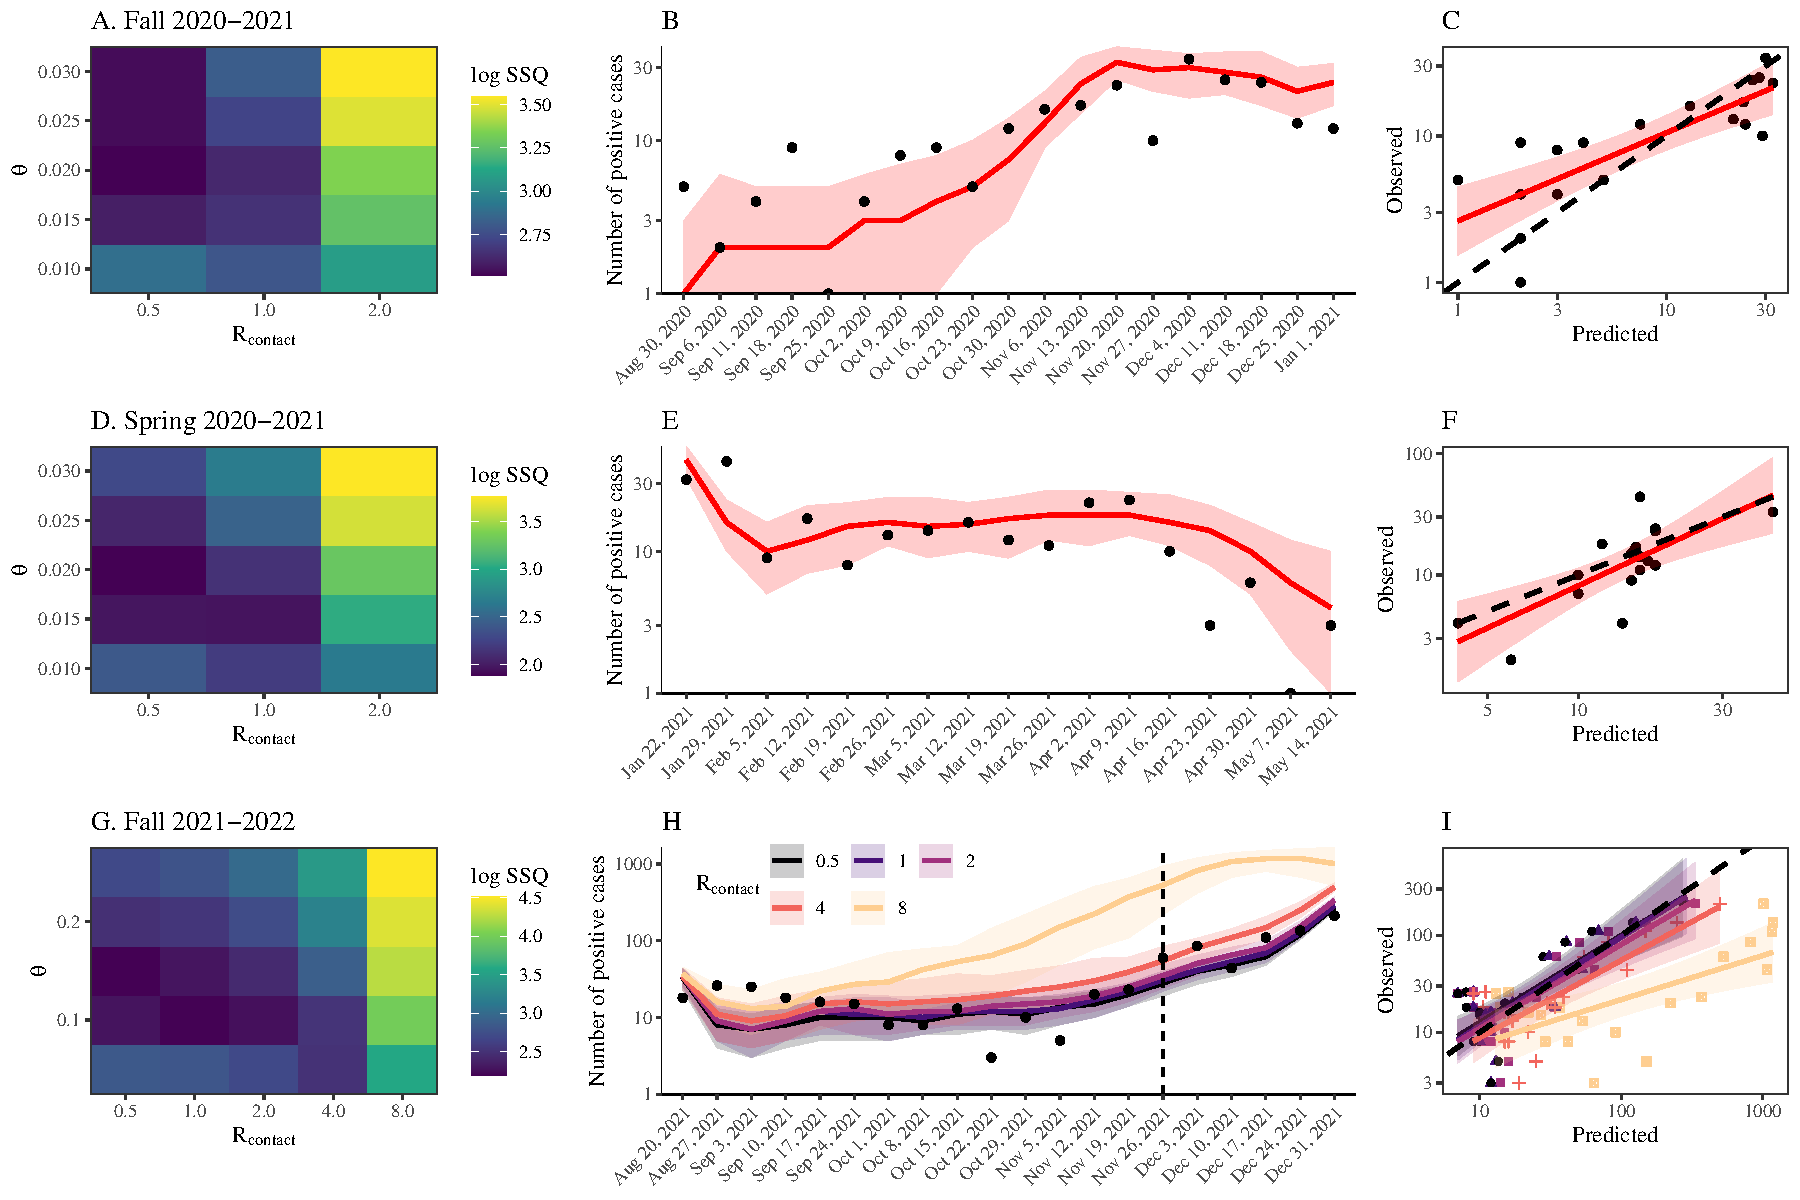
\includegraphics[width=\textwidth]{../figure_princeton/figure_princeton_simulation.pdf}
\caption{
\textbf{Dynamics of SARS-CoV-2 outbreaks in Princeton University}
(A, D, G) Time series comparisons of model predictions with observed data across ranges of effective reproduction number $\mathcal R_e$ and scaling parameter for community transmission $\theta$.
For each parameter combination, we simulate the model 100 times and calculate the sum of squared differences (SSQ) between the reported number of positive cases and the model-predicted number of positive cases. 
Heat maps represent medians of the logged sum of squared differences.
(B, E, H) Model predictions. 
Solid lines represent median predictions.
Shaded areas represent 90\% quantiles for the best matching parameter set.
Points represent the observed data.
(C, F, I) Correlations between model predictions with observed data.
Colored solid lines and shaded areas represent the estimated linear regression lines and the associated 95\% CIs.
Dashed lines represent the one-to-one line.
\label{fig:matching}
}
\end{figure}

We find that a low value of $\mathcal R_e=0.5$ and a small amount of community transmission $\theta=0.015$ is most consistent with the observed epidemic dynamics in fall 2020 (\fref{matching}A).
With these parameters, the model is able to capture the rise and fall in the number of cases with the exception of sudden decrease in the number of cases around Thanksgiving, which we do not model explicitly (\fref{matching}B).
The median predictions are positively correlated with the observed dynamics ($\rho = 0.83$; 95\% CI: 0.61--0.93; \fref{matching}C).
Although a wide range of assumptions about the levels of community transmission $\theta$ are consistent with the observed dynamics, our simulations preclude high $\mathcal R_e > 2$ (SUPP).
Distancing measures on campus and contact tracing efforts likely contributed to lowering $\mathcal R_e$.

A similar set of parameters can capture the observed dynamics in spring 2020.
The best matching parameter predicts a slightly higher levels of community transmission $\theta=0.02$ (\fref{matching}D), but a wide range of parameters are consistent with the observed dynamics as before (SUPP). 
Simulations also preclude high $\mathcal R_e > 2$ again, suggesting that the contact levels between students likely remained low even though they had returned to campus---the absence of in-person teaching is likely to have contributed to lowering $\mathcal R_e$.
Once again, we find a positive (but slightly weaker) correlation between the predicted and the observed numbers of cases ($\rho = 0.62$; 95\% CI: 0.20--0.85; \fref{matching}F).

For fall 2021, we limited our model comparison to November 26th before the Omicron variant was introduced on campus.
We assume that $>95\%$ of the school population is vaccinated at the beginning of the semester and do not model additional doses throughout the semester for simplicity.
We also allow vaccine-derived immunity to wane over time to ask whether the increase in the number of cases around November is consistent with the dynamics predicted by immunity waning.

Even though the numbers of cases during fall 2021 (before a large outbreak) were similar to those during previous semesters, we find that considerably higher levels of community transmission $\theta$ (~10 fold higher) is required to explain the observed dynamics due to a decreased susceptibility from vaccination (\fref{matching}G).
We note that the parameter $\theta$ necessarily depends on our assumed vaccine efficacy, and $\theta$ would decrease if we assume a lower vaccine efficacy.
Nonetheless, the amount of community transmission would still need to be higher than previous semesters as long as vaccine provides some protection against infection.

We also find that the predicted dynamics are largely insensitive to $\mathcal R_e$ until November 26th (\fref{matching}H)---
in addition, all simulations shown in \fref{matching}H are positively correlated with the observed numbers of cases (\fref{matching}G). 
An increasing pattern in the sum of squared errors with $\mathcal R_e$ shown in \fref{matching}G is primarily driven by the discrepancy around fall break (week ending October 26th) when the number of cases decreased suddenly, which we do not model explicitly.
As nearly all school population was vaccinated, transmission between individuals on campus would have been limited, making $\mathcal R_e$ difficult to estimate.
These simulations also suggest that an increase in the number of cases in November can be explained by a combination of waning immunity alone without requiring additional changes in transmission dynamics (note we do not allow $\theta$ or $\mathcal R_e$ to vary over time).

Projecting the model beyond November 26th shows that we would have seen a similarly growth in the number of cases if conditions remained constant even without the introduction of the Omicron variant.
In other words, the Delta strain would have continued to spread on campus at a similar rate if the semester were to (hypothetically) continue until January without additional interventions (\fref{matching}H).
In reality, the situation was more complex:  testing frequencies increased and social gatherings were limited in response to an increase in the number of cases.
These interventions---as well as students returning back home as classes ended---likely would have reduced contact rates (and therefore transmission of the Delta variant).
This reduction in transmission was likely counterbalanced by the introduction of the Omicron variant and its immune evasion, leading to similar and persistent growth in the number of cases.

We then project epidemic trajectories for the spread of the Omicron variant among 4000 students for the spring semester of 2021 across a wide range of effective reproduction number ($\mathcal R_e = 2--16$) and testing frequencies (every 2, 4, and 7 days).
We assume a two-dose efficacy 10\% and a three-dose efficacy of 70\% against the infection and transmission of the Omicron variant. 
We further assume that immunity from the third dose takes 14 days to develop and can wane at the same rate as previously assumed (in this case, 70\% to 39\% in 20 weeks).
For simplicity, we assume a constant amount of external infections.

\fref{omicron} shows predicted trajectories of new infections per day (A) and the mean susceptibility over time (B).
Across a wide range of $\mathcal R_e$, we find that a frequent testing alone is not sufficient to prevent an outbreak---while testing and isolation can prevent onward transmission once infected, it cannot prevent infections from happening especially if they are coming from outside of the population.
Administering booster shots at a faster rate (compare 30 vs 60 booster shots per day in \fref{omicron}A) can help reduce the size of the epidemic peak and cause the epidemic to decay faster, their overall impact is limited due to delays in developing immunity and imperfect protection against the Omicron variant.
Comparing changes in the mean susceptibility further reveal that administering booster shots at a faster rate can also lead to earlier immunity waning and higher mean susceptibility by the end of the semester, which may increase chances of an outbreak in the future \fref{omicron}.

\begin{figure}[!th]
\includegraphics[width=\textwidth]{../figure_omicron/figure_omicron.pdf}
\caption{
\textbf{Scenario projects of the spread of omicron variant on university campus}
(A) The predicted daily number of new infections across a wide ranges assumptions about testing frequencies, effective reproduction number $\mathcal R_e$, and the number of booster shots given per day.
(B) The predicted effective susceptibility over time. 
Effective susceptibility is calculated by taking the mean of individual-level susceptibility of each student.
Solid lines and shaded areas represent the median and the corresponding 90\% quantiles across 100 simulations.
All other parameters are the same as in Figure 2.
\label{fig:omicron}
}
\end{figure}

So far we have assumed that all individuals who test positive are isolated for 10 days;
in practice, however, isolation of infected individuals can be limited by the isolation bed capacity.
As the Omicron variant is expected to spread rapidly on university campuses (\fref{omicron}), universities participating in testing plans can expect to face difficulties in isolating infected individuals.
Here, we explore how limiting the number of isolation beds on university campus can affect epidemic dynamics by assuming that individuals who test positive will not be isolated and will continue to transmit when isolation beds are full.
In doing so, we also consider the effects of shorter isolation periods (5, 7, and 10 days).

\begin{figure}[!th]
\includegraphics[width=\textwidth]{../figure_omicron/figure_omicron_limit.pdf}
\caption{
\textbf{Scenario projects of the spread of omicron variant on university campus with limited isolation beds}
(A) The predicted numbers of individuals in isolation on a given day.
(B) The predicted daily number of new infections.
Solid lines and shaded areas represent the median and the corresponding 90\% quantiles across 100 simulations.
We assume $\mathcal R_0 = 8$, 30 booster shots given per day, and testing frequency of 3 days for these simulations.
All other parameters are the same as in Figure 3.
\label{fig:isolation}
}
\end{figure}

When there are no limits to the number of isolation beds on campus, shortening isolation periods results in a slightly higher number of total infections (\fref{isolation}A): .
The epidemic trajectory remains similar across different values of isolation periods (\fref{isolation}B), but the number of students in isolation becomes considerably lower with shorter isolation periods (\fref{isolation}C).
For example, the maximum number of students in isolation decreases from ??? to ???.

When the number of isolation beds is moderately limited ($=200$), shortening isolation periods can decrease the total numbers of infections (\fref{isolation}A) and considerably reduce the size of the epidemic peak (\fref{isolation}B). 
Even when the number of isolation beds is severely limited ($=100$), shortening isolation periods can still reduce the size of the epidemic peak (\fref{isolation}B) because we are able to isolate a greater proportion of infected individuals and prevent onward transmission.
Longer isolation can prevent a greater amount of onward transmission \emph{per individual} but permits a lower number of individuals in isolation, making it less effectiveness when the number of isolation beds are limited.

\section*{Discussion}

Here, we present the analysis of SARS-CoV-2 outbreaks on Princeton University campus between fall 2020 and early 2022.
Our analysis demonstrates strong spatiotemporal correlations between the patterns of spread of SARS-CoV-2 on university campus and those from surrounding communities.
These correlations decreased with distance from Mercer County in fall 2021, likely reflecting contact and commuting patterns as university re-opened.
Mathematical modeling further suggests limited transmission between the university population during fall and spring semesters of 2020 and an increased amount of community contacts during the fall semester of 2021 compared previous semesters.
An increase in the number of cases by the end of November 2021 is consistent with the increase in the levels of community cases and waning immunity.
Finally, we predict the spread of Omicron variant to likely cause a large outbreak in the spring semester of 2021 even under more stringent testing protocols.
A rapid administration of booster shots and shortening isolation periods can help reduce the size of an outbreak, but uncertainty remains for future semesters.

Previous outbreak reports from other universities primarily focused on transmission on university campuses \citep{wilson2020multiple,currie2021interventions} and provided limited insights into the importance of community transmission in shaping epidemic dynamics.
For example, extensive modeling efforts from Cornell University also demonstrated increase in the amount of transmission from outside the university campus and found that community transmissions are the biggest risk for faculty and staff members \citep{frazier2022modeling};
but they did not demonstrate explicit correlations between university and community cases and further assumed that the amount of community transmission does not change over a semester.
To our knowledge, our analysis is the first to demonstrate a strong spatiotemporal correlation in the spread of SARS-CoV-2 between university campuses and surrounding communities.
Our analysis further indicate that comparing the ratios between the cases on university campuses and neighboring communities can provide a useful measure for how well a university campus might be doing in controlling the epidemic---we note that this ratio need to be interpreted with caution as it is sensitive to changes in testing patterns.

The recent recommendations by the Centers for Disease Control and Prevention to reduce isolation periods from 10 to 5 days \citep{cdcisolation} have generated much discussion regarding its individual- and population-level implications \citep{soljak2022reducing}.
Given uncertainty in the duration of infectiousness of the Omicron variant, shortening the duration of isolation can increase the chances of transmission after infected individuals are released from their isolation---as we also show here, this can lead to an increase in the final size of an outbreak.
When the number of isolation beds are limited, however, shorter isolation periods can help mitigate spread by allowing a greater number of individuals to be isolated.
We note that the net benefits of shortening isolation periods are sensitive to many factors, such as the duration of infectiousness, isolation bed capacity, and time from infection to isolation, which will vary across different universities.
Therefore, caution is needed in implementing these changes in other places.
Incorporating lateral flow tests at the end of isolation can also help prevent excess transmission \citep{quilty2022test}.

There are several limitations to our analysis.
While our analysis demonstrates strong spatiotemporal correlation in the spread of SARS-CoV-2, we are not able to infer the direction of causality---that is, our analysis does not rule out the possibility that transmission on campus drove infections in nearby communities (as opposed to community transmission driving on-campus infections).
Nonetheless, intervention measures on campus (e.g., frequent asymptomatic testing, contact tracing, and virtual classes during fall and spring semesters of 2020) likely limited onward transmission on campus, and therefore, transmission from community to campus is likely to have had greater effects.
Decreasing patterns in epidemic correlations with distance further highlight the role of spatial spread in driving dynamics of SARS-CoV-2---such patterns are consistent with spatial spread of many other respiratory pathogens \citep{grenfell2001travelling, viboud2006synchrony, baker2019epidemic}.

Our mathematical model relies on simplifying assumptions.
For example, we assume that the entire university populations mix homogeneously and have identical campus and community contact rates (captured by $\mathcal R_e$ and $\theta$, respectively).
In reality, increases in cases were often associated with specific transmission clusters, suggesting heterogeneity in transmission patterns.
Contact levels also likely differ between different groups;
for example, faculty and staff members are more likely to interact with community members than undergraduate students and are therefore at a higher risk for community infections \citep{frazier2022modeling}.
We also do not account for changes in behavior. 
Instead, we assume a constant $\theta$ and $\mathcal R_e$ throughout a semester (note this $\mathcal R_e$ implicitly accounts for some interventions, but not for testing or changes in susceptibility driven by vaccination or infection).
We also do not explore parameter uncertainty, which can lead to underestimation of overall uncertainty \citep{elderd2006uncertainty}. 
We also note that intervention measures that were introduced to Princeton University may not necessarily be applicable in other universities.

Despite the simplicity of the analysis, our study provides important lessons for controlling SARS-CoV-2 outbreaks on university campuses in general.
First, the safe reopening of a university campus must consider the spread of SARS-CoV-2 within the surrounding community as they can both drive transmission in each other.
Second, combining multiple interventions measures, such as social distancing, mask wearing, frequent testing, and vaccination, can help provide safe means of re-opening university campuses---
the extent to which these interventions are implemented will necessarily depend on resource availability
Finally, intervention measures placed on campuses must continue to adapt and change to reflect changes in epidemiological conditions.



\bibliography{university-covid}

\pagebreak

\section*{Supplementary Figures}

\begin{figure}[!th]
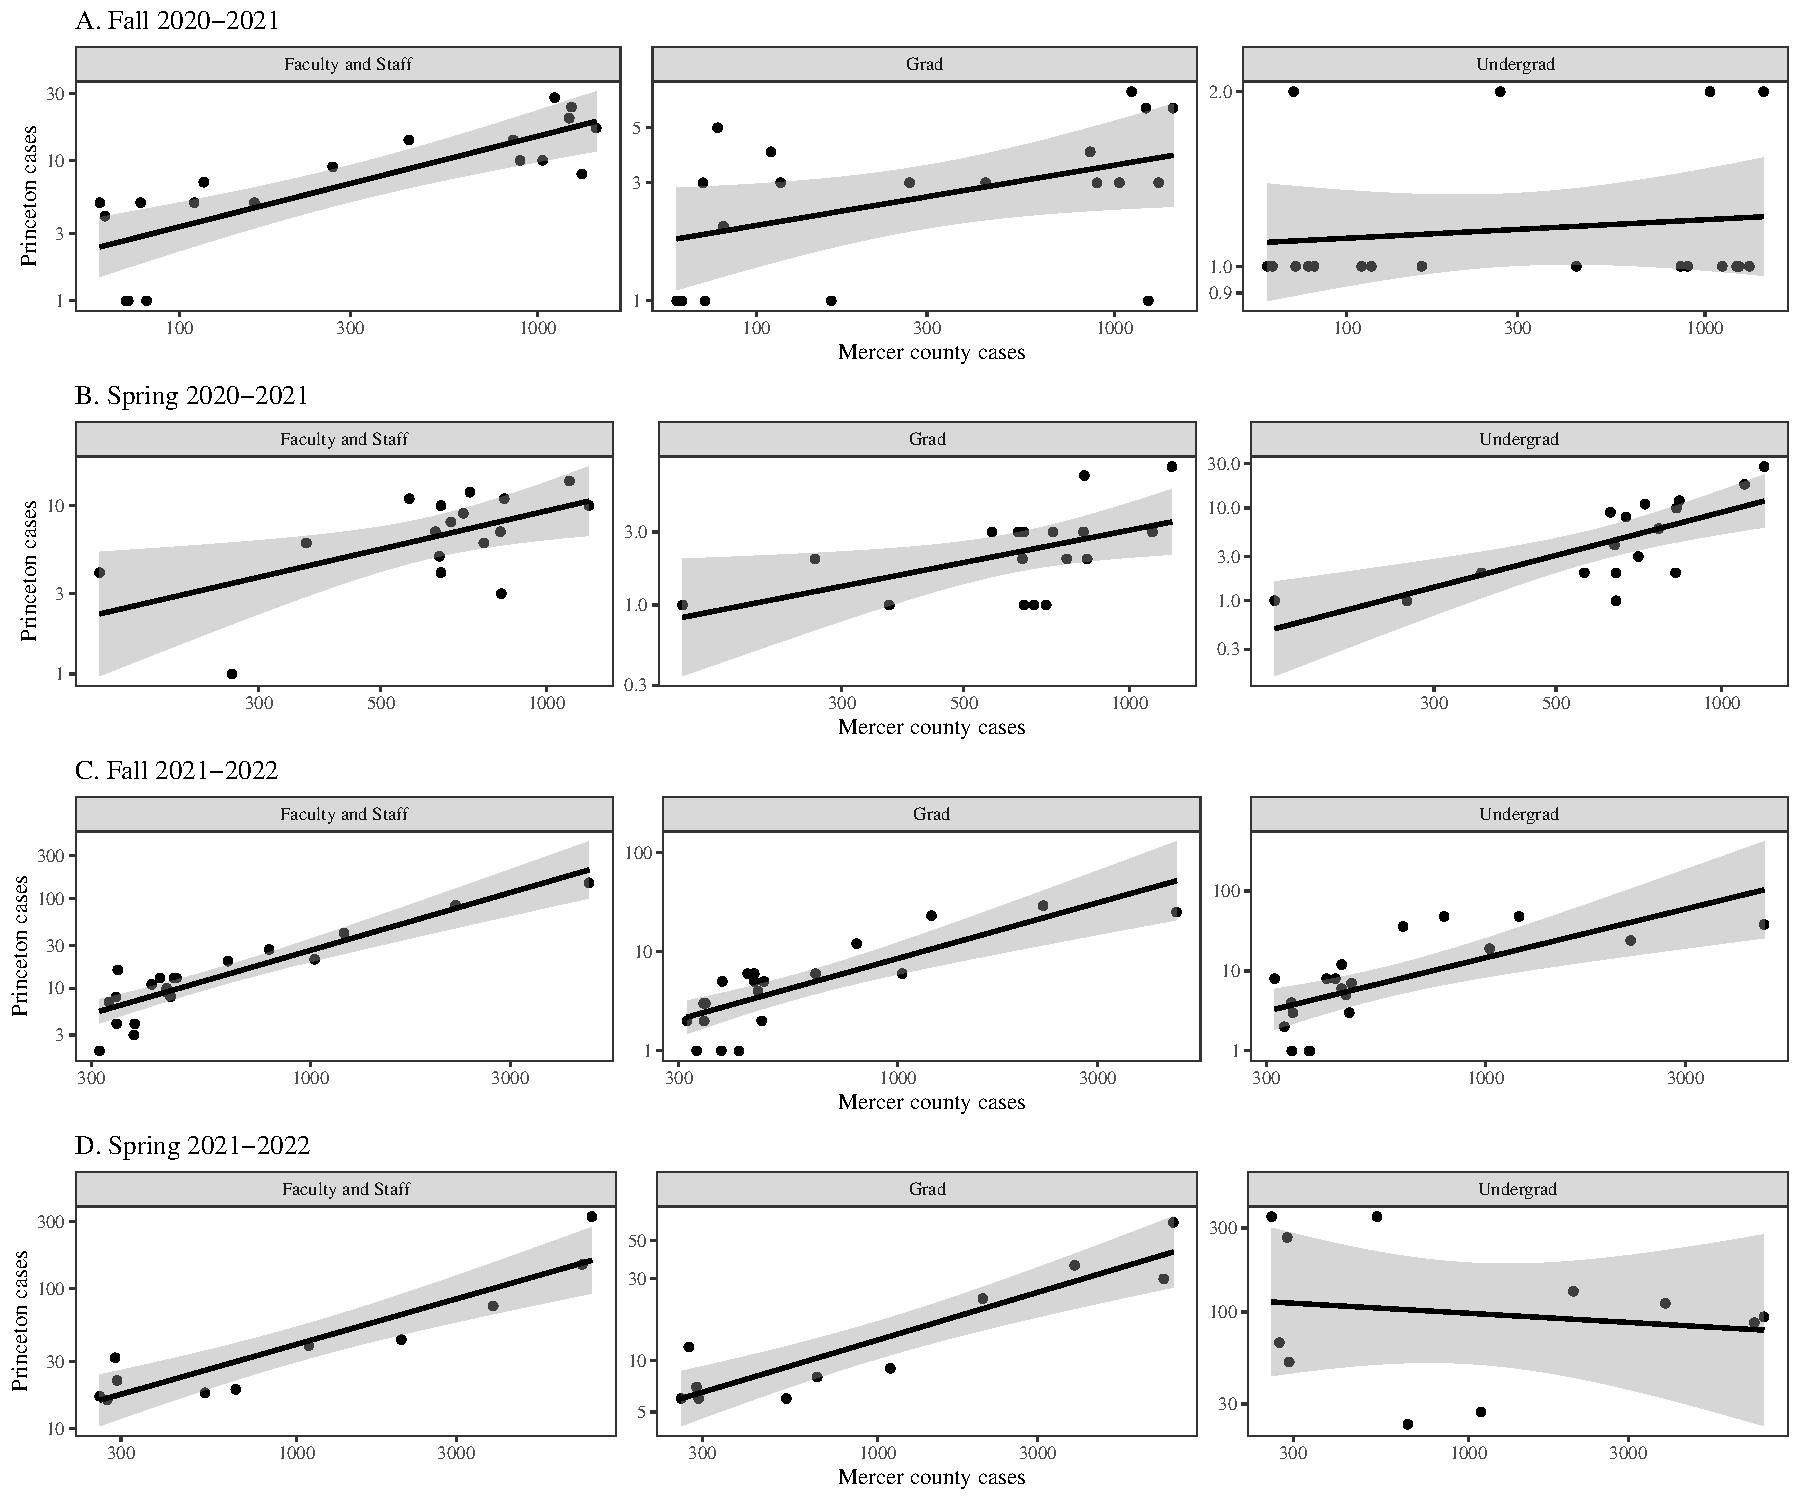
\includegraphics[width=\textwidth]{../figure_princeton/figure_princeton_correlation2.pdf}
\end{figure}

\pagebreak

\begin{figure}[!th]
\includegraphics[width=\textwidth]{../figure_princeton/figure_princeton_map.pdf}
\end{figure}


\pagebreak

\begin{figure}[!th]
\includegraphics[width=\textwidth]{../figure_princeton/figure_princeton_newyork.pdf}
\end{figure}


\pagebreak

\begin{figure}[!th]
\includegraphics[width=\textwidth]{../figure_princeton/figure_princeton_phil.pdf}
\end{figure}


\end{document}
